% Template for PLoS
% Version 3.1 February 2015
%
% To compile to pdf, run:
% latex plos.template
% bibtex plos.template
% latex plos.template
% latex plos.template
% dvipdf plos.template
%
% % % % % % % % % % % % % % % % % % % % % %
%
% -- IMPORTANT NOTE
%
% This template contains comments intended 
% to minimize problems and delays during our production 
% process. Please follow the template instructions
% whenever possible.
%
% % % % % % % % % % % % % % % % % % % % % % % 
%
% Once your paper is accepted for publication, 
% PLEASE REMOVE ALL TRACKED CHANGES in this file and leave only
% the final text of your manuscript.
%
% There are no restrictions on package use within the LaTeX files except that 
% no packages listed in the template may be deleted.
%
% Please do not include colors or graphics in the text.
%
% Please do not create a heading level below \subsection. For 3rd level headings, use \paragraph{}.
%
% % % % % % % % % % % % % % % % % % % % % % %
%
% -- FIGURES AND TABLES
%
% Please include tables/figure captions directly after the paragraph where they are first cited in the text.
%
% DO NOT INCLUDE GRAPHICS IN YOUR MANUSCRIPT
% - Figures should be uploaded separately from your manuscript file. 
% - Figures generated using LaTeX should be extracted and removed from the PDF before submission. 
% - Figures containing multiple panels/subfigures must be combined into one image file before submission.
% For figure citations, please use "Fig." instead of "Figure".
% See http://www.plosone.org/static/figureGuidelines for PLOS figure guidelines.
%
% Tables should be cell-based and may not contain:
% - tabs/spacing/line breaks within cells to alter layout or alignment
% - vertically-merged cells (no tabular environments within tabular environments, do not use \multirow)
% - colors, shading, or graphic objects
% See http://www.plosone.org/static/figureGuidelines#tables for table guidelines.
%
% For tables that exceed the width of the text column, use the adjustwidth environment as illustrated in the example table in text below.
%
% % % % % % % % % % % % % % % % % % % % % % % %
%
% -- EQUATIONS, MATH SYMBOLS, SUBSCRIPTS, AND SUPERSCRIPTS
%
% IMPORTANT
% Below are a few tips to help format your equations and other special characters according to our specifications. For more tips to help reduce the possibility of formatting errors during conversion, please see our LaTeX guidelines at http://www.plosone.org/static/latexGuidelines
%
% Please be sure to include all portions of an equation in the math environment.
%
% Do not include text that is not math in the math environment. For example, CO2 will be CO\textsubscript{2}.
%
% Please add line breaks to long display equations when possible in order to fit size of the column. 
%
% For inline equations, please do not include punctuation (commas, etc) within the math environment unless this is part of the equation.
%
% % % % % % % % % % % % % % % % % % % % % % % % 
%
% Please contact latex@plos.org with any questions.
%
% % % % % % % % % % % % % % % % % % % % % % % %

\documentclass[10pt,letterpaper]{article}
\usepackage[top=0.85in,left=2.75in,footskip=0.75in]{geometry}

% Use adjustwidth environment to exceed column width (see example table in text)
\usepackage{changepage}

% Use Unicode characters when possible
\usepackage[utf8]{inputenc}

% textcomp package and marvosym package for additional characters
\usepackage{textcomp,marvosym}

% fixltx2e package for \textsubscript
\usepackage{fixltx2e}

% amsmath and amssymb packages, useful for mathematical formulas and symbols
\usepackage{amsmath,amssymb}

% cite package, to clean up citations in the main text. Do not remove.
\usepackage{cite}

% Use nameref to cite supporting information files (see Supporting Information section for more info)
\usepackage{nameref,hyperref}

% line numbers
\usepackage[right]{lineno}

% ligatures disabled
\usepackage{microtype}
\DisableLigatures[f]{encoding = *, family = * }

% rotating package for sideways tables
\usepackage{rotating}

% Remove comment for double spacing
%\usepackage{setspace} 
%\doublespacing

% Text layout
\raggedright
\setlength{\parindent}{0.5cm}
\textwidth 5.25in 
\textheight 8.75in

% Bold the 'Figure #' in the caption and separate it from the title/caption with a period
% Captions will be left justified
\usepackage[aboveskip=1pt,labelfont=bf,labelsep=period,justification=raggedright,singlelinecheck=off]{caption}

% Use the PLoS provided BiBTeX style
\bibliographystyle{plos2015}

% Remove brackets from numbering in List of References
\makeatletter
\renewcommand{\@biblabel}[1]{\quad#1.}
\makeatother

% Leave date blank
\date{}

% Header and Footer with logo
\usepackage{lastpage,fancyhdr,graphicx}
\usepackage{epstopdf}
\pagestyle{myheadings}
\pagestyle{fancy}
\fancyhf{}
\lhead{
\includegraphics[width=2.0in]{PLOS-submission.eps}}
\rfoot{\thepage/\pageref{LastPage}}
\renewcommand{\footrule}{\hrule height 2pt \vspace{2mm}}
\fancyheadoffset[L]{2.25in}
\fancyfootoffset[L]{2.25in}
\lfoot{\sf PLOS}

%% Include all macros below

\newcommand{\lorem}{{\bf LOREM}}
\newcommand{\ipsum}{{\bf IPSUM}}

%% END MACROS SECTION


%%%% Additional user-defined macros

%% Math

% Operators
\DeclareMathOperator{\Cov}{Cov}
\DeclareMathOperator{\Var}{Var}
\DeclareMathOperator{\E}{\mathbb{E}}
\DeclareMathOperator{\Proba}{\mathbb{P}}

\newcommand{\Covb}[2]{\ensuremath{\Cov\!\left[#1,#2\right]}}
\newcommand{\Eb}[1]{\ensuremath{\E\!\left[#1\right]}}
\newcommand{\Pb}[1]{\ensuremath{\Proba\!\left[#1\right]}}
\newcommand{\Varb}[1]{\ensuremath{\Var\!\left[#1\right]}}

% norm
\newcommand{\norm}[1]{\| #1 \|}







\begin{document}
\vspace*{0.35in}

% Title must be 250 characters or less.
% Please capitalize all terms in the title except conjunctions, prepositions, and articles.
\begin{flushleft}
{\Large
\textbf\newline{Calibration of a Spatialized Urban Growth Model - Submission to PLOS Journals}
}
\newline
% Insert author names, affiliations and corresponding author email (do not include titles, positions, or degrees).
\\
Raimbault Juste\textsuperscript{1}
\\
\bigskip
\bf{1} UMR CNRS 8504 G{\'e}ographie-cit{\'e}s, Universit{\'e} Paris 7, Paris, France
\\
\bigskip

% Insert additional author notes using the symbols described below. Insert symbol callouts after author names as necessary.
% 
% Remove or comment out the author notes below if they aren't used.
%
% Primary Equal Contribution Note
%\Yinyang These authors contributed equally to this work.

% Additional Equal Contribution Note
% Also use this double-dagger symbol for special authorship notes, such as senior authorship.
%\ddag These authors also contributed equally to this work.

% Current address notes
%\textcurrency a Insert current address of first author with an address update
% \textcurrency b Insert current address of second author with an address update
% \textcurrency c Insert current address of third author with an address update

% Deceased author note
%\dag Deceased

% Group/Consortium Author Note
%\textpilcrow Membership list can be found in the Acknowledgments section.

% Use the asterisk to denote corresponding authorship and provide email address in note below.
* juste.raimbault@parisgeo.cnrs.fr

\end{flushleft}
% Please keep the abstract below 300 words
\section*{Abstract}



We propose a stochastic model of urban growth that generates spatial distributions of population densities, at an intermediate scale between economic models at the macro scale and land-use evolution models focusing on local relations. Integrating simply the two opposite key processes of aggregation (``preferential attachment'') and diffusion (urban sprawl), we show that we can capture the whole spectrum of existing urban forms in Europe. An extensive exploration and calibration of the proposed model allows determining the region of parameter space corresponding morphologically to observed european urban systems, providing an validated thematic interpretation to model parameters, and furthermore determining the effective dimension of the urban system at this scale regarding morphological objectives.





% Please keep the Author Summary between 150 and 200 words
% Use first person. PLOS ONE authors please skip this step. 
% Author Summary not valid for PLOS ONE submissions.   
%\section*{Author Summary}


\linenumbers





%%%%%%%%%%%%%%%%%%%%%%%%
\section*{Introduction}

Urban Systems are complex socio-technical objects




% - > literature on stochastic urban growth, ABM for Urban Growth, CA Models and urban morphogenesis models. Reproducing urban growth at different scales, capturing different processes.
% ⇒ Plus réponse à cette question : pourquoi simuler la croissance urbaine (quels enjeux scientifiques et sociaux ?)

% Macro models (Gibrat and extensions) are partially spatialized (Favaro - Pumain includes distance between cities, Simpops/Marius also) whereas micro (most CA) are ‘’over-spatialized’’ (neighborhood-based).  
% -> Research Question :  What about a simple model at the meso scale, close to macro by the stylized facts (preferential attachment) but producing morphologically consistent spatial distribution of densities ?



\cite{andersson2002urban} propose a micro-based model of urban growth, with the purpose to replace non-interpretable physical mechanisms with agent mechanisms, including interactions forces and mobility choices. Local correlations are used in \cite{makse1998modeling} to modulate growth patterns to ressemble real configurations. In the same spirit, our model situates at similar scales and can be qualified as a morphogenesis model.








%%%%%%%%%%%%%%%%%%%%%%%%
% You may title this section "Methods" or "Models". 
% "Models" is not a valid title for PLoS ONE authors. However, PLoS ONE
% authors may use "Analysis" 
\section*{Materials and Methods}

\subsection*{The urban growth model}




\paragraph{Rationale}

%Preferential attchment and diffusion, extension of [Batty, 2006]. small litt. prefAtt and then Urban sprawl, opposed forces that must shape morphology of urban systems. choice of a scale at which spatial form has a sense but city system is ‘’wide enough” : 50-100km, meso-scale ?


% \cite{2016arXiv160806313S} : how Simon model generates power law (paper more general to be quoted ?) ; first mover : path dependency of obtained shapes.


% following Florent : \cite{fujita1996economics} oppose agglomeration and sprawl

Our model is an extension of the diffusion-limited aggregation model studied in~\cite{batty2006hierarchy}. Indeed, the tension between antagonist aggregation and sprawl mechanisms may be an important process in urban morphogenesis. For example \cite{fujita1996economics} opposes centrifugal forces with centripetal forces in the equilibrium view of urban spatial systems, what is easily transferable to non-equilibrium systems in the framework of self-organized complexity : a urban structure is a far-from-equilibrium system that has been driven to this point by these opposite forces. The two contradictory processes of urban concentration and urban sprawl are captured by the model, what allows to reproduce with a good precision a large number of existing morphologies.


\paragraph{Scale}

% choice of scale : linked to the notion of morphogenesis


\paragraph{Settings}

%Precise formulation, description and formalization of the model. ; parameters and their possible interpretation ; def of parameter space.

The model $D$ proceeds iteratively the following way. An square grid of width $N$, initially empty, is represented by population $(P_i(t))_{1\leq i\leq N^2}$. At each time step, until total population reaches a fixed parameter $P_m$,
\begin{itemize}
\item total population is increased of a fixed number $N_G$ (growth rate), following a preferential attachment such that 
\[\Pb{P_i(t+1)=P_i(t)+1|P(t+1)=P(t)+1}=\frac{(P_i(t)/P(t))^{\alpha}}{\sum(P_i(t)/P(t))^{\alpha}}\]
\item a fraction $\beta$ of population is diffused to four closest neighbors is operated $n_d$ times
\end{itemize}









\subsection*{Indicators}


% Literature on morphological analysis, method taken from [Le Nechet 2015] to qualify/quantify urban form. Why would form be relevant at this scale ? -> thematic references on variety of urban developments, rural settlements, etc. : form translates many spatial processes at this scale. [beware question of equifiniality : model is however themtically-based for processes].


% on other ways to quantify form ? -> ex fractal shape index ; recent research \cite{2016arXiv160808839C}

% Definition of indicators

%Indicators to qualify model outputs are morphological measures of population density, proposed in~\cite{le2015forme}, that are entropy, hierarchy, spatial auto-correlation, mean distance. 


As our model is only density-based, we propose to quantify its outputs through spatial morphology, i.e. characteristics of density spatial distribution. We need therefore quantities having a certain level of robustness and invariance. For example, two polycentric cities should be classified as morphologically close whereas a direct comparison of distributions (Earth Mover Distance e.g.) could give a very high distance between configurations depending on center positions. To tackle this issue, we refer to the Urban Morphology Analysis literature which proposes an extensive set of indicators to describe urban form~\cite{tsai2005quantifying}. The number of dimensions can be reduced to obtain a robust description with a few number of independent indicators~\cite{Schwarz201029}. For the choice of indicators, we follow the analysis done in~\cite{le2015forme} where a typology of large european cities is obtained in consistence with qualitative knowledge. Let denote $(P_i)_{1\leq i \leq N}$ the population of cells, sorted in decreasing order, $d_{ij}$ the distance between cells $i,j$, and $P=\sum_{i=1}^{N} P_i$ total population. The indicators are the following :

\begin{enumerate}
\item Rank-size slope $\gamma$, expressing the degree of hierarchy in the distribution, computed by fitting a power law distribution by $\ln{P_i/P_0} \sim k - \gamma\cdot \ln{i/i_0}$.
\item Distribution Entropy
\[
\mathcal{E} = \sum_{i=1}^{N}\frac{P_i}{P}\cdot \ln{\frac{P_i}{P}}
\]
\item Spatial-autocorrelation given by Moran index, with simple spatial weights given by $w_{ij} = 1/d_{ij}$
\[
r = \frac{\sum_{i\neq j} w_{ij} \left(P_i - \bar{P}\right)\cdot\left(P_j - \bar{P}\right)}{\sum_{i\neq j} w_{ij} \sum_{i}{\left( P_i - \bar{P}\right)}^2}
\]
\item Mean distance between individuals, which gives an idea of population concentration
\[
\bar{d} = 
\]
\end{enumerate}



%%%%%%%%%%%%%%%%%%%%%%%%
% Results and Discussion can be combined.
\section*{Results}


The model was implemented in a first time in NetLogo~\cite{wilensky1999netlogo} for exploration and visualization purposes, later in \texttt{Scala} for performance reasons and easy integration into OpenMole~\cite{reuillon2013openmole} for HPC model exploration. Computation of indicator values on geographical data was done in \texttt{R} using the \texttt{raster} package~\cite{hijmans2015geographic}.




%%%%%%%%%%%%%%%%%%%%%%%%
\subsection*{Generation of urban patterns.}


The model as few parameters but is able to generate a very wide variety of shapes, extending beyond existing forms. In particular, its dynamical nature allows through $P_m$ parameter to choose final regime that can be non-stationarity (generally chaotic shapes), semi-stationarity or total stationarity. Fig.~\ref{fig:densitygeneration} shows examples of generated shapes.




%%%%%%%%%%%%%%%%%%%%%%%%
\subsection*{Model Behavior}

In the study of such a computational model of simulation, the lack of analytical tractability must be balanced by an extensive knowledge 

\paragraph{Convergence}



%convergence properties of indicators ; number of repetitions needed for consistence of results. [histograms and stats of $\sigma$ %TODO]

Indicators show good convergence property and bimodal statistical distribution for cumulated points in the parameter space confirm the existence of superposed regimes : gaussian distribution gives stationary configurations, whereas inverse log-normal distribution are close to real data shape and correspond to non-stationary regime. For one point and a large number of repetitions, we find that 50 repetitions are enough to obtain a 95\% confidence interval smaller than $\sigma$ around indicator mean. 



\paragraph{Exploration of parameter space}

Parameter space is explored using a grid in first experiments, than a Latin Hypercube Sampling exploration. Parameter bounds are $\alpha \in [0.2,2],\beta \in [0,0.1],n_d \in \{0,\ldots , 4\}, N_G \in [500,3000], P_m \in [2000,100000]$. Fig.\ref{fig:densityscatter} shows the result. We also use the parameter space exploration algorithm~\cite{10.1371/journal.pone.0138212} implemented in OpenMole, and obtain in Fig.~\ref{fig:densitypse} the lower bound in Moran-entropy plan, that unexpectedly exhibit a scaling relationship that we aim to explore further.




\paragraph{Statistical analysis.}

% linear regressions to begin with.


%%%%%%%%%%%%%%%%%%%%%%%%
\subsection*{Model Calibration}

\paragraph{Real Data} We use the population density grid provided openly by 


%% Data source (density grid), computation methodology [comparison of sampling/smoothing to avoid bord effects ?] -> reals values of morpho indics on 50kmx50km grids, on all Europe.
%% + summary stats

%Figure : Distributions of indicators values for real dataset of european densities, computed on 50kmx50km grids, with 10km offset to avoid bord effects. [TODO : add log-normal/normal fits ? ]
%  -> cf Empirical Section

Empirical morphological measures for calibration are the one described in the empirical chapter, i.e. the calibration is done on morphological objectives (entropy, hierarchy, spatial auto-correlation, mean distance) against real values computed on the set of 50km sized grid extracted from european density grid~\cite{eurostat}.





\paragraph{Calibration Process}

We use a specific calibration process : a principal component analysis allows to maximize the cumulated distance between generated points and reals points. We select then the point cloud that overlaps real points in the (PC1,PC2) plan, given a distance threshold. Fig.~\ref{fig:densitycalib} shows the points we obtain for four different values of the threshold ranging from $10^{-6}$ to $10^{-3}$.




%%%%%%%%%%%%%%%
\begin{figure}
%\hspace{-2cm}
%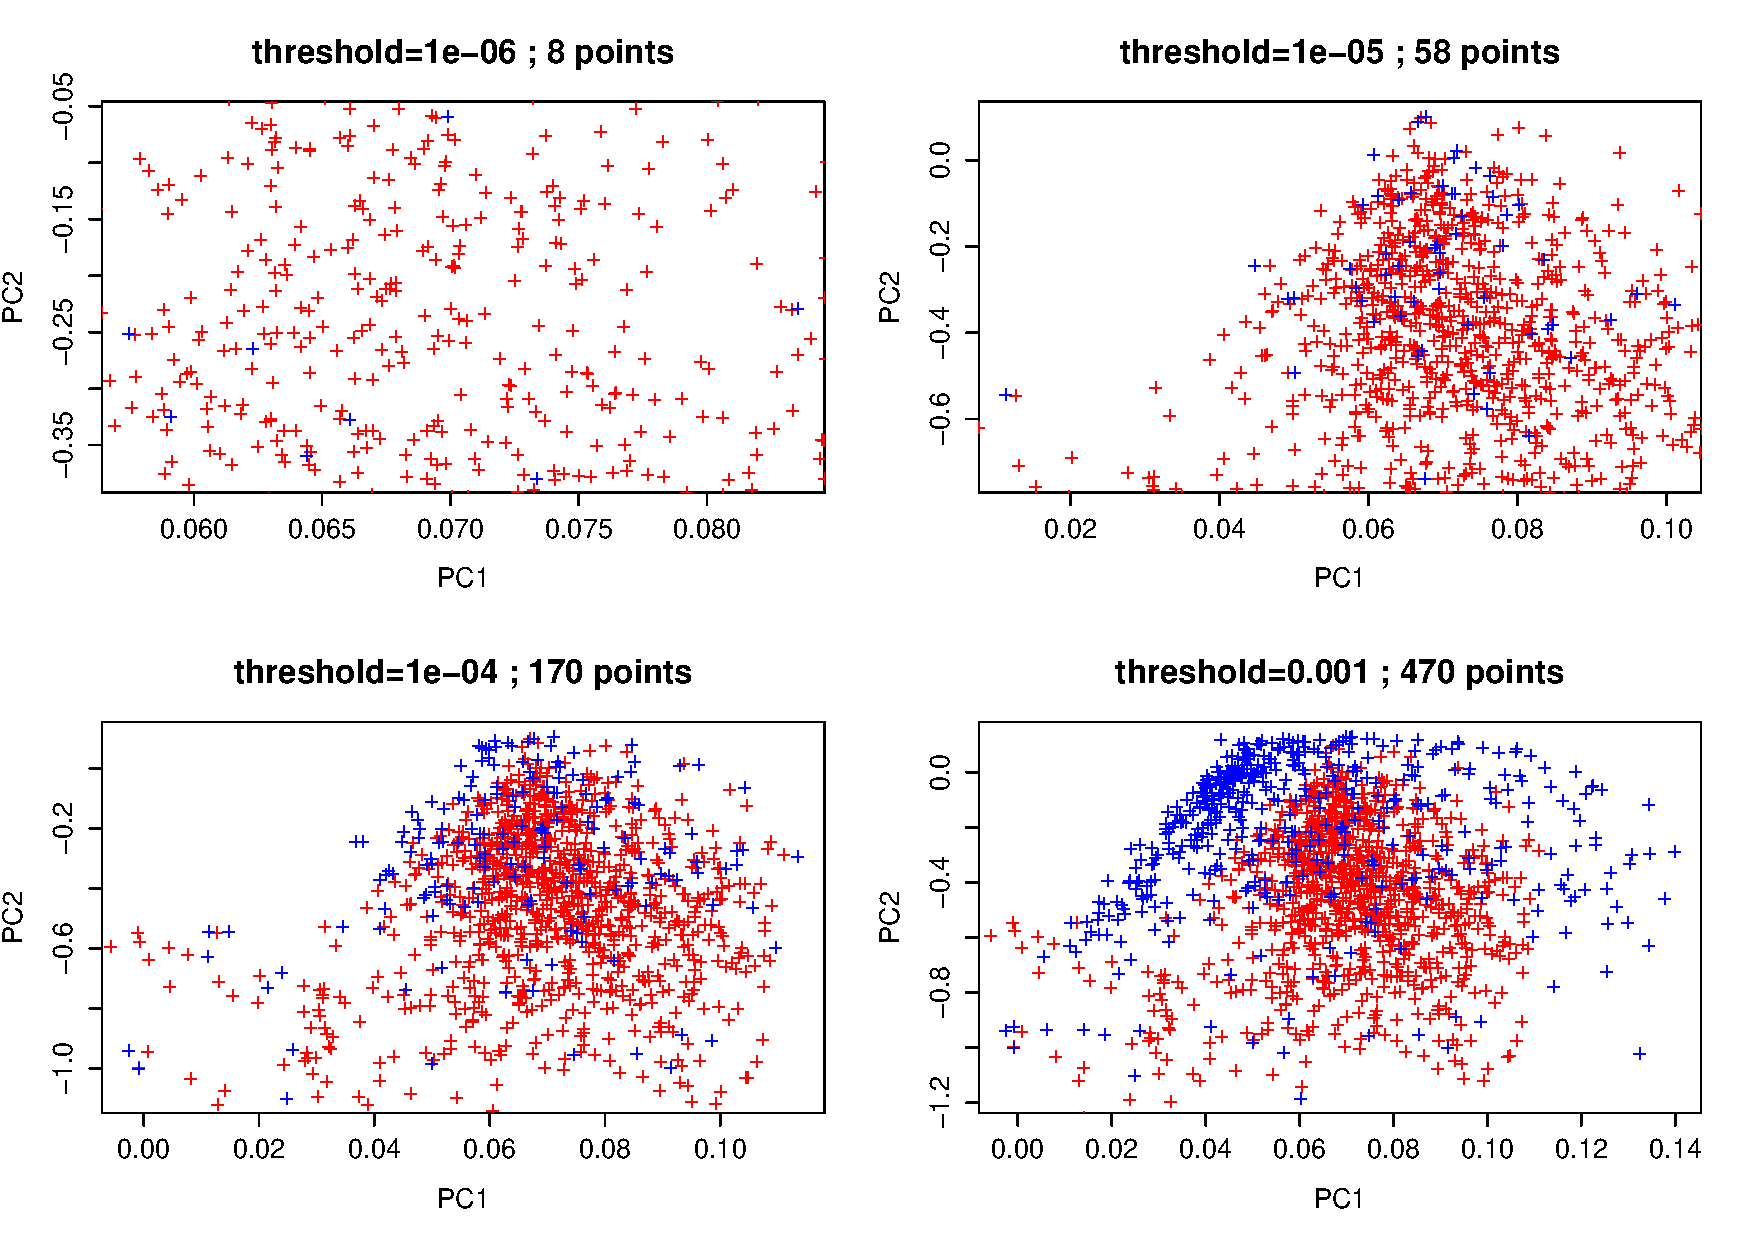
\includegraphics[width=\textwidth]{Figures/PartII/Modeling/UrbanGrowth/pcaDiff_thresholds}
\caption[Precise calibration of the model]{\textbf{Precise calibration of the model.} The principal component analysis is conducted to maximize the spread of the differences between real data and model output, i.e. on the set $\{\left|R_i - M_j\right|\}$ where $R_i$ is the set of real points, $M_j$ the set of model outputs. We select then the overlapping cloud at threshold $\theta$, by taking models output closer to real point cloud than $\theta$ in the (PC1,PC2) plan.}
\label{fig:densitycalib}
\end{figure}
%%%%%%%%%%%%%%





% 3.3.3 - Calibration Results
\paragraph{Calibration refinement}

We plan in further work to extract the exact parameter space covering all real situations and provide interpretation of its shape (correlations between parameters). Its volume in different directions should give the relative importance of parameters.

%[possible development : application of Calibration Profile algo to check relative influence of parameters + ad hoc linear algebra on regression of 3.2.3 to do the same]




%%%%%%%%%%%%%%%%%%%%%%%%
\section*{Discussion}


%%%%%%%%%%%%%%%%%%%%%%%%
\subsection*{Thematic interpretation of growth behavior}

We still need to interpret the positions of typical shapes within parameter space in order to confirm the thematic interpretation of parameters. Depending on results of calibration refinement, we may obtain necessary and sufficient parameters to explain growth at this scale and a corresponding interpretation.



%%%%%%%%%%%%%%%%%%%%%%%%
\subsection*{Integration into a multi-scale growth model}

It could be possible to couple this model with a Gibrat (or Favaro-pumain) at Europa scale (macro) (with addition of consistence on migration constraints), where meso growth rates which were exogenous before are top-down determined, and bottom-up feedback is done through local aggregation level, influence importance of each area.




%%%%%%%%%%%%%%%%%%%%%%%%
\section*{Conclusion}




%%%%%%%%%%%%%%%%%%%%%%%%
\section*{Supporting Information}

% Include only the SI item label in the subsection heading. Use the \nameref{label} command to cite SI items in the text.
\subsection*{S1 Figure}
\label{S1_Figure}
{\bf Bold the first sentence.}



%%%%%%%%%%%%%%%%%%%%%%%%
\section*{Acknowledgments}



\nolinenumbers

%\section*{References}
% Either type in your references using
% \begin{thebibliography}{}
% \bibitem{}
% Text
% \end{thebibliography}
%
% OR
%
% Compile your BiBTeX database using our plos2015.bst
% style file and paste the contents of your .bbl file
% here.
% 


\bibliographystyle{plos2015}
\bibliography{/Users/Juste/Documents/ComplexSystems/CityNetwork/Biblio/Bibtex/CityNetwork}

%
%\begin{thebibliography}{1}
%
%\bibitem{tsai2005quantifying}
%Tsai YH.
%\newblock Quantifying urban form: compactness versus' sprawl'.
%\newblock Urban studies. 2005;42(1):141--161.
%
%\bibitem{Schwarz201029}
%Schwarz N.
%\newblock Urban form revisited---Selecting indicators for characterising
%  European cities.
%\newblock Landscape and Urban Planning. 2010;96(1):29 -- 47.
%\newblock Available from:
%  \url{http://www.sciencedirect.com/science/article/pii/S0169204610000320}.
%
%\bibitem{le2015forme}
%Le~N{\'e}chet F.
%\newblock De la forme urbaine {\`a} la structure m{\'e}tropolitaine: une
%  typologie de la configuration interne des densit{\'e}s pour les principales
%  m{\'e}tropoles europ{\'e}ennes de l'Audit Urbain.
%\newblock Cybergeo: European Journal of Geography. 2015;.
%
%\bibitem{wilensky1999netlogo}
%Wilensky U.
%\newblock NetLogo. 1999;.
%
%\end{thebibliography}






%%%%%%%%%%%%%% Tab template %%%%%%%%%%%%%%%%

%\begin{table}[!ht]
%\begin{adjustwidth}{-2.25in}{0in} % Comment out/remove adjustwidth environment if table fits in text column.
%\caption{
%{\bf Table caption Nulla mi mi, venenatis sed ipsum varius, volutpat euismod diam.}}
%\begin{tabular}{|l|l|l|l|l|l|l|l|}
%\hline
%\multicolumn{4}{|l|}{\bf Heading1} & \multicolumn{4}{|l|}{\bf Heading2}\\ \hline
%$cell1 row1$ & cell2 row 1 & cell3 row 1 & cell4 row 1 & cell5 row 1 & cell6 row 1 & cell7 row 1 & cell8 row 1\\ \hline
%$cell1 row2$ & cell2 row 2 & cell3 row 2 & cell4 row 2 & cell5 row 2 & cell6 row 2 & cell7 row 2 & cell8 row 2\\ \hline
%$cell1 row3$ & cell2 row 3 & cell3 row 3 & cell4 row 3 & cell5 row 3 & cell6 row 3 & cell7 row 3 & cell8 row 3\\ \hline
%\end{tabular}
%\begin{flushleft} Table notes Phasellus venenatis, tortor nec vestibulum mattis, massa tortor interdum felis, nec pellentesque metus tortor nec nisl. Ut ornare mauris tellus, vel dapibus arcu suscipit sed.
%\end{flushleft}
%\label{table1}
%\end{adjustwidth}
%\end{table}


%%%%%%%%%%%%% Fig. Template %%%%%%%%%%%%%%%%%

%\begin{figure}[h]
%\caption{{\bf Figure Title first bold sentence Nulla mi mi, venenatis sed ipsum varius, volutpat euismod diam.}
%Figure Caption Proin rutrum vel massa non gravida. Quisque tempor sem et dignissim rutrum. A: Lorem ipsum dolor sit amet. B: Consectetur adipiscing elit.}
%\label{fig1}
%\end{figure}




%%%%%%%%%%%%%% Eq. Template %%%%%%%%%%%%%%%%%

%\begin{equation}\label{eq:schemeP} 
%D_{coll} = \frac{D_f+\frac{[S]^2}{K_D S_T} D_S} {1+\frac{[S]^2}{K_D S_T}}, 
%D_{sm} = \frac{D_f+ \frac{[S]}{K_D} D_S}{1+\frac{[S]}{K_D}},
%\end{equation}





\end{document}

